% Created by tikzDevice version 0.12.3.1 on 2021-07-02 12:57:45
% !TEX encoding = UTF-8 Unicode
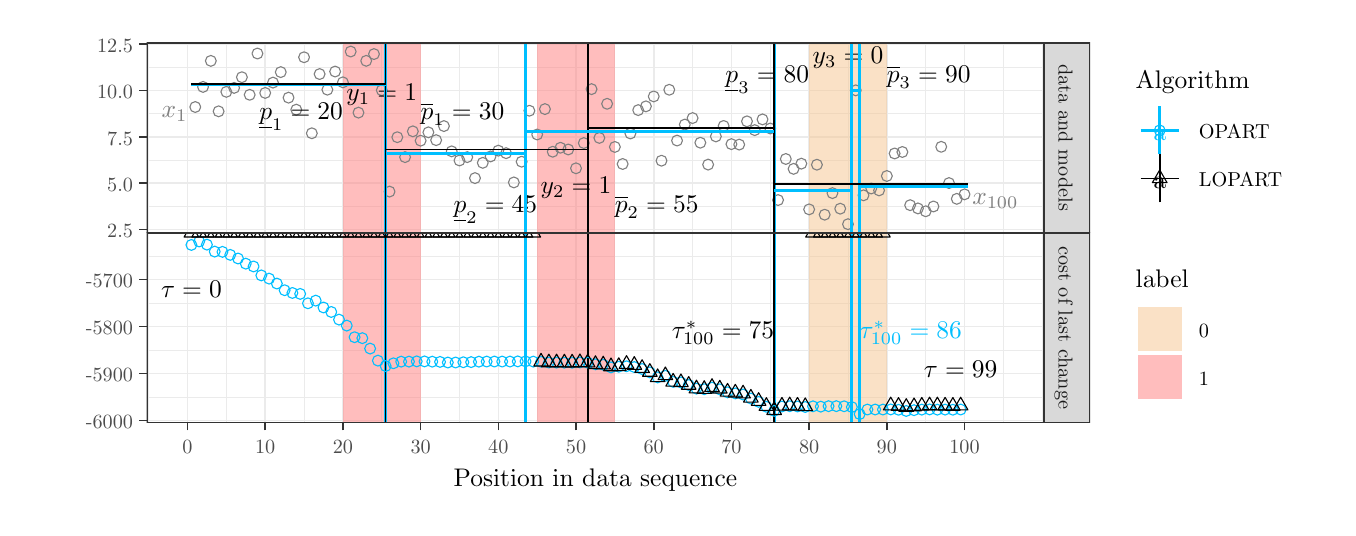
\begin{tikzpicture}[x=1pt,y=1pt]
\definecolor{fillColor}{RGB}{255,255,255}
\path[use as bounding box,fill=fillColor,fill opacity=0.00] (0,0) rectangle (469.75,173.45);
\begin{scope}
\path[clip] (  0.00,  0.00) rectangle (469.75,173.45);
\definecolor{drawColor}{RGB}{255,255,255}
\definecolor{fillColor}{RGB}{255,255,255}

\path[draw=drawColor,line width= 0.6pt,line join=round,line cap=round,fill=fillColor] (  0.00,  0.00) rectangle (469.76,173.45);
\end{scope}
\begin{scope}
\path[clip] ( 43.01, 99.32) rectangle (367.31,167.95);
\definecolor{fillColor}{RGB}{255,255,255}

\path[fill=fillColor] ( 43.01, 99.32) rectangle (367.31,167.95);
\definecolor{drawColor}{gray}{0.92}

\path[draw=drawColor,line width= 0.3pt,line join=round] ( 43.01,108.86) --
	(367.31,108.86);

\path[draw=drawColor,line width= 0.3pt,line join=round] ( 43.01,125.64) --
	(367.31,125.64);

\path[draw=drawColor,line width= 0.3pt,line join=round] ( 43.01,142.41) --
	(367.31,142.41);

\path[draw=drawColor,line width= 0.3pt,line join=round] ( 43.01,159.19) --
	(367.31,159.19);

\path[draw=drawColor,line width= 0.3pt,line join=round] ( 43.72, 99.32) --
	( 43.72,167.95);

\path[draw=drawColor,line width= 0.3pt,line join=round] ( 71.79, 99.32) --
	( 71.79,167.95);

\path[draw=drawColor,line width= 0.3pt,line join=round] ( 99.87, 99.32) --
	( 99.87,167.95);

\path[draw=drawColor,line width= 0.3pt,line join=round] (127.95, 99.32) --
	(127.95,167.95);

\path[draw=drawColor,line width= 0.3pt,line join=round] (156.03, 99.32) --
	(156.03,167.95);

\path[draw=drawColor,line width= 0.3pt,line join=round] (184.11, 99.32) --
	(184.11,167.95);

\path[draw=drawColor,line width= 0.3pt,line join=round] (212.18, 99.32) --
	(212.18,167.95);

\path[draw=drawColor,line width= 0.3pt,line join=round] (240.26, 99.32) --
	(240.26,167.95);

\path[draw=drawColor,line width= 0.3pt,line join=round] (268.34, 99.32) --
	(268.34,167.95);

\path[draw=drawColor,line width= 0.3pt,line join=round] (296.42, 99.32) --
	(296.42,167.95);

\path[draw=drawColor,line width= 0.3pt,line join=round] (324.49, 99.32) --
	(324.49,167.95);

\path[draw=drawColor,line width= 0.3pt,line join=round] (352.57, 99.32) --
	(352.57,167.95);

\path[draw=drawColor,line width= 0.3pt,line join=round] (366.61, 99.32) --
	(366.61,167.95);

\path[draw=drawColor,line width= 0.6pt,line join=round] ( 43.01,100.48) --
	(367.31,100.48);

\path[draw=drawColor,line width= 0.6pt,line join=round] ( 43.01,117.25) --
	(367.31,117.25);

\path[draw=drawColor,line width= 0.6pt,line join=round] ( 43.01,134.03) --
	(367.31,134.03);

\path[draw=drawColor,line width= 0.6pt,line join=round] ( 43.01,150.80) --
	(367.31,150.80);

\path[draw=drawColor,line width= 0.6pt,line join=round] ( 43.01,167.57) --
	(367.31,167.57);

\path[draw=drawColor,line width= 0.6pt,line join=round] ( 57.76, 99.32) --
	( 57.76,167.95);

\path[draw=drawColor,line width= 0.6pt,line join=round] ( 85.83, 99.32) --
	( 85.83,167.95);

\path[draw=drawColor,line width= 0.6pt,line join=round] (113.91, 99.32) --
	(113.91,167.95);

\path[draw=drawColor,line width= 0.6pt,line join=round] (141.99, 99.32) --
	(141.99,167.95);

\path[draw=drawColor,line width= 0.6pt,line join=round] (170.07, 99.32) --
	(170.07,167.95);

\path[draw=drawColor,line width= 0.6pt,line join=round] (198.14, 99.32) --
	(198.14,167.95);

\path[draw=drawColor,line width= 0.6pt,line join=round] (226.22, 99.32) --
	(226.22,167.95);

\path[draw=drawColor,line width= 0.6pt,line join=round] (254.30, 99.32) --
	(254.30,167.95);

\path[draw=drawColor,line width= 0.6pt,line join=round] (282.38, 99.32) --
	(282.38,167.95);

\path[draw=drawColor,line width= 0.6pt,line join=round] (310.46, 99.32) --
	(310.46,167.95);

\path[draw=drawColor,line width= 0.6pt,line join=round] (338.53, 99.32) --
	(338.53,167.95);
\definecolor{drawColor}{gray}{0.50}

\node[text=drawColor,anchor=base east,inner sep=0pt, outer sep=0pt, scale=  0.92] at ( 57.76,140.98) {$x_{1}$};

\node[text=drawColor,anchor=base west,inner sep=0pt, outer sep=0pt, scale=  0.92] at (341.34,109.42) {$x_{100}$};
\definecolor{fillColor}{RGB}{255,125,125}

\path[fill=fillColor,fill opacity=0.50] (113.91, 99.32) rectangle (141.99,167.95);

\path[fill=fillColor,fill opacity=0.50] (184.11, 99.32) rectangle (212.18,167.95);
\definecolor{fillColor}{RGB}{246,196,143}

\path[fill=fillColor,fill opacity=0.50] (282.38, 99.32) rectangle (310.46,167.95);

\path[draw=drawColor,line width= 0.4pt,line join=round,line cap=round] ( 60.56,144.78) circle (  1.96);

\path[draw=drawColor,line width= 0.4pt,line join=round,line cap=round] ( 63.37,152.04) circle (  1.96);

\path[draw=drawColor,line width= 0.4pt,line join=round,line cap=round] ( 66.18,161.45) circle (  1.96);

\path[draw=drawColor,line width= 0.4pt,line join=round,line cap=round] ( 68.99,143.22) circle (  1.96);

\path[draw=drawColor,line width= 0.4pt,line join=round,line cap=round] ( 71.79,150.26) circle (  1.96);

\path[draw=drawColor,line width= 0.4pt,line join=round,line cap=round] ( 74.60,151.69) circle (  1.96);

\path[draw=drawColor,line width= 0.4pt,line join=round,line cap=round] ( 77.41,155.55) circle (  1.96);

\path[draw=drawColor,line width= 0.4pt,line join=round,line cap=round] ( 80.22,149.19) circle (  1.96);

\path[draw=drawColor,line width= 0.4pt,line join=round,line cap=round] ( 83.03,164.11) circle (  1.96);

\path[draw=drawColor,line width= 0.4pt,line join=round,line cap=round] ( 85.83,149.87) circle (  1.96);

\path[draw=drawColor,line width= 0.4pt,line join=round,line cap=round] ( 88.64,153.60) circle (  1.96);

\path[draw=drawColor,line width= 0.4pt,line join=round,line cap=round] ( 91.45,157.39) circle (  1.96);

\path[draw=drawColor,line width= 0.4pt,line join=round,line cap=round] ( 94.26,148.16) circle (  1.96);

\path[draw=drawColor,line width= 0.4pt,line join=round,line cap=round] ( 97.06,143.82) circle (  1.96);

\path[draw=drawColor,line width= 0.4pt,line join=round,line cap=round] ( 99.87,162.76) circle (  1.96);

\path[draw=drawColor,line width= 0.4pt,line join=round,line cap=round] (102.68,135.29) circle (  1.96);

\path[draw=drawColor,line width= 0.4pt,line join=round,line cap=round] (105.49,156.69) circle (  1.96);

\path[draw=drawColor,line width= 0.4pt,line join=round,line cap=round] (108.30,151.04) circle (  1.96);

\path[draw=drawColor,line width= 0.4pt,line join=round,line cap=round] (111.10,157.60) circle (  1.96);

\path[draw=drawColor,line width= 0.4pt,line join=round,line cap=round] (113.91,153.70) circle (  1.96);

\path[draw=drawColor,line width= 0.4pt,line join=round,line cap=round] (116.72,164.83) circle (  1.96);

\path[draw=drawColor,line width= 0.4pt,line join=round,line cap=round] (119.53,142.75) circle (  1.96);

\path[draw=drawColor,line width= 0.4pt,line join=round,line cap=round] (122.33,161.47) circle (  1.96);

\path[draw=drawColor,line width= 0.4pt,line join=round,line cap=round] (125.14,163.91) circle (  1.96);

\path[draw=drawColor,line width= 0.4pt,line join=round,line cap=round] (127.95,150.83) circle (  1.96);

\path[draw=drawColor,line width= 0.4pt,line join=round,line cap=round] (130.76,114.22) circle (  1.96);

\path[draw=drawColor,line width= 0.4pt,line join=round,line cap=round] (133.57,133.87) circle (  1.96);

\path[draw=drawColor,line width= 0.4pt,line join=round,line cap=round] (136.37,126.67) circle (  1.96);

\path[draw=drawColor,line width= 0.4pt,line join=round,line cap=round] (139.18,135.99) circle (  1.96);

\path[draw=drawColor,line width= 0.4pt,line join=round,line cap=round] (141.99,132.61) circle (  1.96);

\path[draw=drawColor,line width= 0.4pt,line join=round,line cap=round] (144.80,135.63) circle (  1.96);

\path[draw=drawColor,line width= 0.4pt,line join=round,line cap=round] (147.60,132.81) circle (  1.96);

\path[draw=drawColor,line width= 0.4pt,line join=round,line cap=round] (150.41,137.89) circle (  1.96);

\path[draw=drawColor,line width= 0.4pt,line join=round,line cap=round] (153.22,128.76) circle (  1.96);

\path[draw=drawColor,line width= 0.4pt,line join=round,line cap=round] (156.03,125.46) circle (  1.96);

\path[draw=drawColor,line width= 0.4pt,line join=round,line cap=round] (158.84,126.67) circle (  1.96);

\path[draw=drawColor,line width= 0.4pt,line join=round,line cap=round] (161.64,119.09) circle (  1.96);

\path[draw=drawColor,line width= 0.4pt,line join=round,line cap=round] (164.45,124.61) circle (  1.96);

\path[draw=drawColor,line width= 0.4pt,line join=round,line cap=round] (167.26,126.92) circle (  1.96);

\path[draw=drawColor,line width= 0.4pt,line join=round,line cap=round] (170.07,129.02) circle (  1.96);

\path[draw=drawColor,line width= 0.4pt,line join=round,line cap=round] (172.87,128.10) circle (  1.96);

\path[draw=drawColor,line width= 0.4pt,line join=round,line cap=round] (175.68,117.53) circle (  1.96);

\path[draw=drawColor,line width= 0.4pt,line join=round,line cap=round] (178.49,125.02) circle (  1.96);

\path[draw=drawColor,line width= 0.4pt,line join=round,line cap=round] (181.30,143.44) circle (  1.96);

\path[draw=drawColor,line width= 0.4pt,line join=round,line cap=round] (184.11,134.85) circle (  1.96);

\path[draw=drawColor,line width= 0.4pt,line join=round,line cap=round] (186.91,144.03) circle (  1.96);

\path[draw=drawColor,line width= 0.4pt,line join=round,line cap=round] (189.72,128.62) circle (  1.96);

\path[draw=drawColor,line width= 0.4pt,line join=round,line cap=round] (192.53,130.06) circle (  1.96);

\path[draw=drawColor,line width= 0.4pt,line join=round,line cap=round] (195.34,129.43) circle (  1.96);

\path[draw=drawColor,line width= 0.4pt,line join=round,line cap=round] (198.14,122.63) circle (  1.96);

\path[draw=drawColor,line width= 0.4pt,line join=round,line cap=round] (200.95,131.76) circle (  1.96);

\path[draw=drawColor,line width= 0.4pt,line join=round,line cap=round] (203.76,151.24) circle (  1.96);

\path[draw=drawColor,line width= 0.4pt,line join=round,line cap=round] (206.57,133.61) circle (  1.96);

\path[draw=drawColor,line width= 0.4pt,line join=round,line cap=round] (209.38,145.94) circle (  1.96);

\path[draw=drawColor,line width= 0.4pt,line join=round,line cap=round] (212.18,130.35) circle (  1.96);

\path[draw=drawColor,line width= 0.4pt,line join=round,line cap=round] (214.99,124.19) circle (  1.96);

\path[draw=drawColor,line width= 0.4pt,line join=round,line cap=round] (217.80,135.21) circle (  1.96);

\path[draw=drawColor,line width= 0.4pt,line join=round,line cap=round] (220.61,143.66) circle (  1.96);

\path[draw=drawColor,line width= 0.4pt,line join=round,line cap=round] (223.41,145.02) circle (  1.96);

\path[draw=drawColor,line width= 0.4pt,line join=round,line cap=round] (226.22,148.60) circle (  1.96);

\path[draw=drawColor,line width= 0.4pt,line join=round,line cap=round] (229.03,125.38) circle (  1.96);

\path[draw=drawColor,line width= 0.4pt,line join=round,line cap=round] (231.84,151.01) circle (  1.96);

\path[draw=drawColor,line width= 0.4pt,line join=round,line cap=round] (234.65,132.66) circle (  1.96);

\path[draw=drawColor,line width= 0.4pt,line join=round,line cap=round] (237.45,138.44) circle (  1.96);

\path[draw=drawColor,line width= 0.4pt,line join=round,line cap=round] (240.26,140.78) circle (  1.96);

\path[draw=drawColor,line width= 0.4pt,line join=round,line cap=round] (243.07,131.88) circle (  1.96);

\path[draw=drawColor,line width= 0.4pt,line join=round,line cap=round] (245.88,123.97) circle (  1.96);

\path[draw=drawColor,line width= 0.4pt,line join=round,line cap=round] (248.68,134.16) circle (  1.96);

\path[draw=drawColor,line width= 0.4pt,line join=round,line cap=round] (251.49,137.94) circle (  1.96);

\path[draw=drawColor,line width= 0.4pt,line join=round,line cap=round] (254.30,131.37) circle (  1.96);

\path[draw=drawColor,line width= 0.4pt,line join=round,line cap=round] (257.11,131.20) circle (  1.96);

\path[draw=drawColor,line width= 0.4pt,line join=round,line cap=round] (259.92,139.60) circle (  1.96);

\path[draw=drawColor,line width= 0.4pt,line join=round,line cap=round] (262.72,136.43) circle (  1.96);

\path[draw=drawColor,line width= 0.4pt,line join=round,line cap=round] (265.53,140.30) circle (  1.96);

\path[draw=drawColor,line width= 0.4pt,line join=round,line cap=round] (268.34,137.02) circle (  1.96);

\path[draw=drawColor,line width= 0.4pt,line join=round,line cap=round] (271.15,111.16) circle (  1.96);

\path[draw=drawColor,line width= 0.4pt,line join=round,line cap=round] (273.95,126.00) circle (  1.96);

\path[draw=drawColor,line width= 0.4pt,line join=round,line cap=round] (276.76,122.43) circle (  1.96);

\path[draw=drawColor,line width= 0.4pt,line join=round,line cap=round] (279.57,124.31) circle (  1.96);

\path[draw=drawColor,line width= 0.4pt,line join=round,line cap=round] (282.38,107.79) circle (  1.96);

\path[draw=drawColor,line width= 0.4pt,line join=round,line cap=round] (285.19,123.93) circle (  1.96);

\path[draw=drawColor,line width= 0.4pt,line join=round,line cap=round] (287.99,105.87) circle (  1.96);

\path[draw=drawColor,line width= 0.4pt,line join=round,line cap=round] (290.80,113.67) circle (  1.96);

\path[draw=drawColor,line width= 0.4pt,line join=round,line cap=round] (293.61,108.04) circle (  1.96);

\path[draw=drawColor,line width= 0.4pt,line join=round,line cap=round] (296.42,102.44) circle (  1.96);

\path[draw=drawColor,line width= 0.4pt,line join=round,line cap=round] (299.22,150.80) circle (  1.96);

\path[draw=drawColor,line width= 0.4pt,line join=round,line cap=round] (302.03,112.87) circle (  1.96);

\path[draw=drawColor,line width= 0.4pt,line join=round,line cap=round] (304.84,115.34) circle (  1.96);

\path[draw=drawColor,line width= 0.4pt,line join=round,line cap=round] (307.65,114.65) circle (  1.96);

\path[draw=drawColor,line width= 0.4pt,line join=round,line cap=round] (310.46,119.85) circle (  1.96);

\path[draw=drawColor,line width= 0.4pt,line join=round,line cap=round] (313.26,127.99) circle (  1.96);

\path[draw=drawColor,line width= 0.4pt,line join=round,line cap=round] (316.07,128.53) circle (  1.96);

\path[draw=drawColor,line width= 0.4pt,line join=round,line cap=round] (318.88,109.31) circle (  1.96);

\path[draw=drawColor,line width= 0.4pt,line join=round,line cap=round] (321.69,108.14) circle (  1.96);

\path[draw=drawColor,line width= 0.4pt,line join=round,line cap=round] (324.49,107.10) circle (  1.96);

\path[draw=drawColor,line width= 0.4pt,line join=round,line cap=round] (327.30,108.84) circle (  1.96);

\path[draw=drawColor,line width= 0.4pt,line join=round,line cap=round] (330.11,130.40) circle (  1.96);

\path[draw=drawColor,line width= 0.4pt,line join=round,line cap=round] (332.92,117.30) circle (  1.96);

\path[draw=drawColor,line width= 0.4pt,line join=round,line cap=round] (335.73,111.60) circle (  1.96);

\path[draw=drawColor,line width= 0.4pt,line join=round,line cap=round] (338.53,113.22) circle (  1.96);
\definecolor{drawColor}{RGB}{0,0,0}

\node[text=drawColor,anchor=base east,inner sep=0pt, outer sep=0pt, scale=  0.92] at (113.91,140.29) {$\underline p_{1}=20$};

\node[text=drawColor,anchor=base east,inner sep=0pt, outer sep=0pt, scale=  0.92] at (184.11,106.74) {$\underline p_{2}=45$};

\node[text=drawColor,anchor=base east,inner sep=0pt, outer sep=0pt, scale=  0.92] at (282.38,153.71) {$\underline p_{3}=80$};

\node[text=drawColor,anchor=base,inner sep=0pt, outer sep=0pt, scale=  0.92] at (127.95,147.00) {$y_{1}=1$};

\node[text=drawColor,anchor=base,inner sep=0pt, outer sep=0pt, scale=  0.92] at (198.14,113.45) {$y_{2}=1$};

\node[text=drawColor,anchor=base,inner sep=0pt, outer sep=0pt, scale=  0.92] at (296.42,160.42) {$y_{3}=0$};

\node[text=drawColor,anchor=base west,inner sep=0pt, outer sep=0pt, scale=  0.92] at (141.99,140.29) {$\overline p_{1}=30$};

\node[text=drawColor,anchor=base west,inner sep=0pt, outer sep=0pt, scale=  0.92] at (212.18,106.74) {$\overline p_{2}=55$};

\node[text=drawColor,anchor=base west,inner sep=0pt, outer sep=0pt, scale=  0.92] at (310.46,153.71) {$\overline p_{3}=90$};
\definecolor{drawColor}{RGB}{0,191,255}

\path[draw=drawColor,line width= 1.1pt,line join=round] (129.35, 99.32) -- (129.35,167.95);

\path[draw=drawColor,line width= 1.1pt,line join=round] (179.89, 99.32) -- (179.89,167.95);

\path[draw=drawColor,line width= 1.1pt,line join=round] (269.74, 99.32) -- (269.74,167.95);

\path[draw=drawColor,line width= 1.1pt,line join=round] (297.82, 99.32) -- (297.82,167.95);

\path[draw=drawColor,line width= 1.1pt,line join=round] (300.63, 99.32) -- (300.63,167.95);
\definecolor{drawColor}{RGB}{0,0,0}

\path[draw=drawColor,line width= 0.6pt,line join=round] (129.35, 99.32) -- (129.35,167.95);

\path[draw=drawColor,line width= 0.6pt,line join=round] (202.36, 99.32) -- (202.36,167.95);

\path[draw=drawColor,line width= 0.6pt,line join=round] (269.74, 99.32) -- (269.74,167.95);
\definecolor{drawColor}{RGB}{0,191,255}

\path[draw=drawColor,line width= 1.1pt,line join=round] ( 59.16,153.04) -- (129.35,153.04);

\path[draw=drawColor,line width= 1.1pt,line join=round] (129.35,127.83) -- (179.89,127.83);

\path[draw=drawColor,line width= 1.1pt,line join=round] (179.89,136.09) -- (269.74,136.09);

\path[draw=drawColor,line width= 1.1pt,line join=round] (269.74,114.57) -- (297.82,114.57);

\path[draw=drawColor,line width= 1.1pt,line join=round] (297.82,150.80) -- (300.63,150.80);

\path[draw=drawColor,line width= 1.1pt,line join=round] (300.63,116.08) -- (339.94,116.08);
\definecolor{drawColor}{RGB}{0,0,0}

\path[draw=drawColor,line width= 0.6pt,line join=round] ( 59.16,153.04) -- (129.35,153.04);

\path[draw=drawColor,line width= 0.6pt,line join=round] (129.35,129.45) -- (202.36,129.45);

\path[draw=drawColor,line width= 0.6pt,line join=round] (202.36,137.08) -- (269.74,137.08);

\path[draw=drawColor,line width= 0.6pt,line join=round] (269.74,116.86) -- (339.94,116.86);
\definecolor{drawColor}{gray}{0.20}

\path[draw=drawColor,line width= 0.6pt,line join=round,line cap=round] ( 43.01, 99.32) rectangle (367.31,167.95);
\end{scope}
\begin{scope}
\path[clip] ( 43.01, 30.69) rectangle (367.31, 99.32);
\definecolor{fillColor}{RGB}{255,255,255}

\path[fill=fillColor] ( 43.01, 30.69) rectangle (367.31, 99.32);
\definecolor{drawColor}{gray}{0.92}

\path[draw=drawColor,line width= 0.3pt,line join=round] ( 43.01, 39.97) --
	(367.31, 39.97);

\path[draw=drawColor,line width= 0.3pt,line join=round] ( 43.01, 56.97) --
	(367.31, 56.97);

\path[draw=drawColor,line width= 0.3pt,line join=round] ( 43.01, 73.97) --
	(367.31, 73.97);

\path[draw=drawColor,line width= 0.3pt,line join=round] ( 43.01, 90.96) --
	(367.31, 90.96);

\path[draw=drawColor,line width= 0.3pt,line join=round] ( 43.72, 30.69) --
	( 43.72, 99.32);

\path[draw=drawColor,line width= 0.3pt,line join=round] ( 71.79, 30.69) --
	( 71.79, 99.32);

\path[draw=drawColor,line width= 0.3pt,line join=round] ( 99.87, 30.69) --
	( 99.87, 99.32);

\path[draw=drawColor,line width= 0.3pt,line join=round] (127.95, 30.69) --
	(127.95, 99.32);

\path[draw=drawColor,line width= 0.3pt,line join=round] (156.03, 30.69) --
	(156.03, 99.32);

\path[draw=drawColor,line width= 0.3pt,line join=round] (184.11, 30.69) --
	(184.11, 99.32);

\path[draw=drawColor,line width= 0.3pt,line join=round] (212.18, 30.69) --
	(212.18, 99.32);

\path[draw=drawColor,line width= 0.3pt,line join=round] (240.26, 30.69) --
	(240.26, 99.32);

\path[draw=drawColor,line width= 0.3pt,line join=round] (268.34, 30.69) --
	(268.34, 99.32);

\path[draw=drawColor,line width= 0.3pt,line join=round] (296.42, 30.69) --
	(296.42, 99.32);

\path[draw=drawColor,line width= 0.3pt,line join=round] (324.49, 30.69) --
	(324.49, 99.32);

\path[draw=drawColor,line width= 0.3pt,line join=round] (352.57, 30.69) --
	(352.57, 99.32);

\path[draw=drawColor,line width= 0.3pt,line join=round] (366.61, 30.69) --
	(366.61, 99.32);

\path[draw=drawColor,line width= 0.6pt,line join=round] ( 43.01, 31.48) --
	(367.31, 31.48);

\path[draw=drawColor,line width= 0.6pt,line join=round] ( 43.01, 48.47) --
	(367.31, 48.47);

\path[draw=drawColor,line width= 0.6pt,line join=round] ( 43.01, 65.47) --
	(367.31, 65.47);

\path[draw=drawColor,line width= 0.6pt,line join=round] ( 43.01, 82.47) --
	(367.31, 82.47);

\path[draw=drawColor,line width= 0.6pt,line join=round] ( 57.76, 30.69) --
	( 57.76, 99.32);

\path[draw=drawColor,line width= 0.6pt,line join=round] ( 85.83, 30.69) --
	( 85.83, 99.32);

\path[draw=drawColor,line width= 0.6pt,line join=round] (113.91, 30.69) --
	(113.91, 99.32);

\path[draw=drawColor,line width= 0.6pt,line join=round] (141.99, 30.69) --
	(141.99, 99.32);

\path[draw=drawColor,line width= 0.6pt,line join=round] (170.07, 30.69) --
	(170.07, 99.32);

\path[draw=drawColor,line width= 0.6pt,line join=round] (198.14, 30.69) --
	(198.14, 99.32);

\path[draw=drawColor,line width= 0.6pt,line join=round] (226.22, 30.69) --
	(226.22, 99.32);

\path[draw=drawColor,line width= 0.6pt,line join=round] (254.30, 30.69) --
	(254.30, 99.32);

\path[draw=drawColor,line width= 0.6pt,line join=round] (282.38, 30.69) --
	(282.38, 99.32);

\path[draw=drawColor,line width= 0.6pt,line join=round] (310.46, 30.69) --
	(310.46, 99.32);

\path[draw=drawColor,line width= 0.6pt,line join=round] (338.53, 30.69) --
	(338.53, 99.32);
\definecolor{fillColor}{RGB}{255,125,125}

\path[fill=fillColor,fill opacity=0.50] (113.91, 30.69) rectangle (141.99, 99.32);

\path[fill=fillColor,fill opacity=0.50] (184.11, 30.69) rectangle (212.18, 99.32);
\definecolor{fillColor}{RGB}{246,196,143}

\path[fill=fillColor,fill opacity=0.50] (282.38, 30.69) rectangle (310.46, 99.32);
\definecolor{drawColor}{RGB}{0,191,255}

\path[draw=drawColor,line width= 1.1pt,line join=round] (129.35, 30.69) -- (129.35, 99.32);

\path[draw=drawColor,line width= 1.1pt,line join=round] (179.89, 30.69) -- (179.89, 99.32);

\path[draw=drawColor,line width= 1.1pt,line join=round] (269.74, 30.69) -- (269.74, 99.32);

\path[draw=drawColor,line width= 1.1pt,line join=round] (297.82, 30.69) -- (297.82, 99.32);

\path[draw=drawColor,line width= 1.1pt,line join=round] (300.63, 30.69) -- (300.63, 99.32);
\definecolor{drawColor}{RGB}{0,0,0}

\path[draw=drawColor,line width= 0.6pt,line join=round] (129.35, 30.69) -- (129.35, 99.32);

\path[draw=drawColor,line width= 0.6pt,line join=round] (202.36, 30.69) -- (202.36, 99.32);

\path[draw=drawColor,line width= 0.6pt,line join=round] (269.74, 30.69) -- (269.74, 99.32);

\node[text=drawColor,anchor=base,inner sep=0pt, outer sep=0pt, scale=  0.92] at ( 59.16, 75.93) {$\tau = 0$};

\node[text=drawColor,anchor=base,inner sep=0pt, outer sep=0pt, scale=  0.92] at (337.13, 46.88) {$\tau = 99$};
\definecolor{drawColor}{RGB}{0,191,255}

\node[text=drawColor,anchor=base west,inner sep=0pt, outer sep=0pt, scale=  0.92] at (300.63, 61.20) {$\tau^*_{100} = 86$};
\definecolor{drawColor}{RGB}{0,0,0}

\node[text=drawColor,anchor=base east,inner sep=0pt, outer sep=0pt, scale=  0.92] at (269.74, 61.20) {$\tau^*_{100} = 75$};
\definecolor{drawColor}{RGB}{0,191,255}

\path[draw=drawColor,line width= 0.4pt,line join=round,line cap=round] ( 59.16, 94.94) circle (  1.96);

\path[draw=drawColor,line width= 0.4pt,line join=round,line cap=round] ( 61.97, 96.20) circle (  1.96);

\path[draw=drawColor,line width= 0.4pt,line join=round,line cap=round] ( 64.77, 95.05) circle (  1.96);

\path[draw=drawColor,line width= 0.4pt,line join=round,line cap=round] ( 67.58, 92.54) circle (  1.96);

\path[draw=drawColor,line width= 0.4pt,line join=round,line cap=round] ( 70.39, 92.44) circle (  1.96);

\path[draw=drawColor,line width= 0.4pt,line join=round,line cap=round] ( 73.20, 91.35) circle (  1.96);

\path[draw=drawColor,line width= 0.4pt,line join=round,line cap=round] ( 76.01, 90.04) circle (  1.96);

\path[draw=drawColor,line width= 0.4pt,line join=round,line cap=round] ( 78.81, 88.18) circle (  1.96);

\path[draw=drawColor,line width= 0.4pt,line join=round,line cap=round] ( 81.62, 87.16) circle (  1.96);

\path[draw=drawColor,line width= 0.4pt,line join=round,line cap=round] ( 84.43, 83.93) circle (  1.96);

\path[draw=drawColor,line width= 0.4pt,line join=round,line cap=round] ( 87.24, 82.77) circle (  1.96);

\path[draw=drawColor,line width= 0.4pt,line join=round,line cap=round] ( 90.04, 80.99) circle (  1.96);

\path[draw=drawColor,line width= 0.4pt,line join=round,line cap=round] ( 92.85, 78.58) circle (  1.96);

\path[draw=drawColor,line width= 0.4pt,line join=round,line cap=round] ( 95.66, 77.59) circle (  1.96);

\path[draw=drawColor,line width= 0.4pt,line join=round,line cap=round] ( 98.47, 77.25) circle (  1.96);

\path[draw=drawColor,line width= 0.4pt,line join=round,line cap=round] (101.28, 73.85) circle (  1.96);

\path[draw=drawColor,line width= 0.4pt,line join=round,line cap=round] (104.08, 74.82) circle (  1.96);

\path[draw=drawColor,line width= 0.4pt,line join=round,line cap=round] (106.89, 72.34) circle (  1.96);

\path[draw=drawColor,line width= 0.4pt,line join=round,line cap=round] (109.70, 70.72) circle (  1.96);

\path[draw=drawColor,line width= 0.4pt,line join=round,line cap=round] (112.51, 67.96) circle (  1.96);

\path[draw=drawColor,line width= 0.4pt,line join=round,line cap=round] (115.31, 65.79) circle (  1.96);

\path[draw=drawColor,line width= 0.4pt,line join=round,line cap=round] (118.12, 61.60) circle (  1.96);

\path[draw=drawColor,line width= 0.4pt,line join=round,line cap=round] (120.93, 61.25) circle (  1.96);

\path[draw=drawColor,line width= 0.4pt,line join=round,line cap=round] (123.74, 57.49) circle (  1.96);

\path[draw=drawColor,line width= 0.4pt,line join=round,line cap=round] (126.55, 53.14) circle (  1.96);

\path[draw=drawColor,line width= 0.4pt,line join=round,line cap=round] (129.35, 51.17) circle (  1.96);

\path[draw=drawColor,line width= 0.4pt,line join=round,line cap=round] (132.16, 52.17) circle (  1.96);

\path[draw=drawColor,line width= 0.4pt,line join=round,line cap=round] (134.97, 52.77) circle (  1.96);

\path[draw=drawColor,line width= 0.4pt,line join=round,line cap=round] (137.78, 52.78) circle (  1.96);

\path[draw=drawColor,line width= 0.4pt,line join=round,line cap=round] (140.58, 52.87) circle (  1.96);

\path[draw=drawColor,line width= 0.4pt,line join=round,line cap=round] (143.39, 52.85) circle (  1.96);

\path[draw=drawColor,line width= 0.4pt,line join=round,line cap=round] (146.20, 52.76) circle (  1.96);

\path[draw=drawColor,line width= 0.4pt,line join=round,line cap=round] (149.01, 52.68) circle (  1.96);

\path[draw=drawColor,line width= 0.4pt,line join=round,line cap=round] (151.82, 52.45) circle (  1.96);

\path[draw=drawColor,line width= 0.4pt,line join=round,line cap=round] (154.62, 52.46) circle (  1.96);

\path[draw=drawColor,line width= 0.4pt,line join=round,line cap=round] (157.43, 52.55) circle (  1.96);

\path[draw=drawColor,line width= 0.4pt,line join=round,line cap=round] (160.24, 52.60) circle (  1.96);

\path[draw=drawColor,line width= 0.4pt,line join=round,line cap=round] (163.05, 52.76) circle (  1.96);

\path[draw=drawColor,line width= 0.4pt,line join=round,line cap=round] (165.85, 52.80) circle (  1.96);

\path[draw=drawColor,line width= 0.4pt,line join=round,line cap=round] (168.66, 52.81) circle (  1.96);

\path[draw=drawColor,line width= 0.4pt,line join=round,line cap=round] (171.47, 52.80) circle (  1.96);

\path[draw=drawColor,line width= 0.4pt,line join=round,line cap=round] (174.28, 52.80) circle (  1.96);

\path[draw=drawColor,line width= 0.4pt,line join=round,line cap=round] (177.09, 52.86) circle (  1.96);

\path[draw=drawColor,line width= 0.4pt,line join=round,line cap=round] (179.89, 52.87) circle (  1.96);

\path[draw=drawColor,line width= 0.4pt,line join=round,line cap=round] (182.70, 52.78) circle (  1.96);

\path[draw=drawColor,line width= 0.4pt,line join=round,line cap=round] (185.51, 52.71) circle (  1.96);

\path[draw=drawColor,line width= 0.4pt,line join=round,line cap=round] (188.32, 52.44) circle (  1.96);

\path[draw=drawColor,line width= 0.4pt,line join=round,line cap=round] (191.12, 52.43) circle (  1.96);

\path[draw=drawColor,line width= 0.4pt,line join=round,line cap=round] (193.93, 52.39) circle (  1.96);

\path[draw=drawColor,line width= 0.4pt,line join=round,line cap=round] (196.74, 52.37) circle (  1.96);

\path[draw=drawColor,line width= 0.4pt,line join=round,line cap=round] (199.55, 52.48) circle (  1.96);

\path[draw=drawColor,line width= 0.4pt,line join=round,line cap=round] (202.36, 52.41) circle (  1.96);

\path[draw=drawColor,line width= 0.4pt,line join=round,line cap=round] (205.16, 51.80) circle (  1.96);

\path[draw=drawColor,line width= 0.4pt,line join=round,line cap=round] (207.97, 51.66) circle (  1.96);

\path[draw=drawColor,line width= 0.4pt,line join=round,line cap=round] (210.78, 50.69) circle (  1.96);

\path[draw=drawColor,line width= 0.4pt,line join=round,line cap=round] (213.59, 50.94) circle (  1.96);

\path[draw=drawColor,line width= 0.4pt,line join=round,line cap=round] (216.39, 51.10) circle (  1.96);

\path[draw=drawColor,line width= 0.4pt,line join=round,line cap=round] (219.20, 50.81) circle (  1.96);

\path[draw=drawColor,line width= 0.4pt,line join=round,line cap=round] (222.01, 50.11) circle (  1.96);

\path[draw=drawColor,line width= 0.4pt,line join=round,line cap=round] (224.82, 48.89) circle (  1.96);

\path[draw=drawColor,line width= 0.4pt,line join=round,line cap=round] (227.63, 47.08) circle (  1.96);

\path[draw=drawColor,line width= 0.4pt,line join=round,line cap=round] (230.43, 47.65) circle (  1.96);

\path[draw=drawColor,line width= 0.4pt,line join=round,line cap=round] (233.24, 45.46) circle (  1.96);

\path[draw=drawColor,line width= 0.4pt,line join=round,line cap=round] (236.05, 45.26) circle (  1.96);

\path[draw=drawColor,line width= 0.4pt,line join=round,line cap=round] (238.86, 44.32) circle (  1.96);

\path[draw=drawColor,line width= 0.4pt,line join=round,line cap=round] (241.66, 43.02) circle (  1.96);

\path[draw=drawColor,line width= 0.4pt,line join=round,line cap=round] (244.47, 42.81) circle (  1.96);

\path[draw=drawColor,line width= 0.4pt,line join=round,line cap=round] (247.28, 43.37) circle (  1.96);

\path[draw=drawColor,line width= 0.4pt,line join=round,line cap=round] (250.09, 42.76) circle (  1.96);

\path[draw=drawColor,line width= 0.4pt,line join=round,line cap=round] (252.90, 41.67) circle (  1.96);

\path[draw=drawColor,line width= 0.4pt,line join=round,line cap=round] (255.70, 41.29) circle (  1.96);

\path[draw=drawColor,line width= 0.4pt,line join=round,line cap=round] (258.51, 40.90) circle (  1.96);

\path[draw=drawColor,line width= 0.4pt,line join=round,line cap=round] (261.32, 39.43) circle (  1.96);

\path[draw=drawColor,line width= 0.4pt,line join=round,line cap=round] (264.13, 38.25) circle (  1.96);

\path[draw=drawColor,line width= 0.4pt,line join=round,line cap=round] (266.93, 36.46) circle (  1.96);

\path[draw=drawColor,line width= 0.4pt,line join=round,line cap=round] (269.74, 34.99) circle (  1.96);

\path[draw=drawColor,line width= 0.4pt,line join=round,line cap=round] (272.55, 36.56) circle (  1.96);

\path[draw=drawColor,line width= 0.4pt,line join=round,line cap=round] (275.36, 36.66) circle (  1.96);

\path[draw=drawColor,line width= 0.4pt,line join=round,line cap=round] (278.17, 36.57) circle (  1.96);

\path[draw=drawColor,line width= 0.4pt,line join=round,line cap=round] (280.97, 36.38) circle (  1.96);

\path[draw=drawColor,line width= 0.4pt,line join=round,line cap=round] (283.78, 36.63) circle (  1.96);

\path[draw=drawColor,line width= 0.4pt,line join=round,line cap=round] (286.59, 36.51) circle (  1.96);

\path[draw=drawColor,line width= 0.4pt,line join=round,line cap=round] (289.40, 36.68) circle (  1.96);

\path[draw=drawColor,line width= 0.4pt,line join=round,line cap=round] (292.20, 36.69) circle (  1.96);

\path[draw=drawColor,line width= 0.4pt,line join=round,line cap=round] (295.01, 36.64) circle (  1.96);

\path[draw=drawColor,line width= 0.4pt,line join=round,line cap=round] (297.82, 36.35) circle (  1.96);

\path[draw=drawColor,line width= 0.4pt,line join=round,line cap=round] (300.63, 33.81) circle (  1.96);

\path[draw=drawColor,line width= 0.4pt,line join=round,line cap=round] (303.44, 35.46) circle (  1.96);

\path[draw=drawColor,line width= 0.4pt,line join=round,line cap=round] (306.24, 35.47) circle (  1.96);

\path[draw=drawColor,line width= 0.4pt,line join=round,line cap=round] (309.05, 35.46) circle (  1.96);

\path[draw=drawColor,line width= 0.4pt,line join=round,line cap=round] (311.86, 35.50) circle (  1.96);

\path[draw=drawColor,line width= 0.4pt,line join=round,line cap=round] (314.67, 35.38) circle (  1.96);

\path[draw=drawColor,line width= 0.4pt,line join=round,line cap=round] (317.47, 34.94) circle (  1.96);

\path[draw=drawColor,line width= 0.4pt,line join=round,line cap=round] (320.28, 35.23) circle (  1.96);

\path[draw=drawColor,line width= 0.4pt,line join=round,line cap=round] (323.09, 35.43) circle (  1.96);

\path[draw=drawColor,line width= 0.4pt,line join=round,line cap=round] (325.90, 35.50) circle (  1.96);

\path[draw=drawColor,line width= 0.4pt,line join=round,line cap=round] (328.71, 35.42) circle (  1.96);

\path[draw=drawColor,line width= 0.4pt,line join=round,line cap=round] (331.51, 35.44) circle (  1.96);

\path[draw=drawColor,line width= 0.4pt,line join=round,line cap=round] (334.32, 35.39) circle (  1.96);

\path[draw=drawColor,line width= 0.4pt,line join=round,line cap=round] (337.13, 35.47) circle (  1.96);
\definecolor{drawColor}{RGB}{0,0,0}

\path[draw=drawColor,line width= 0.4pt,line join=round,line cap=round] ( 59.16,102.37) --
	( 61.80, 97.79) --
	( 56.52, 97.79) --
	cycle;

\path[draw=drawColor,line width= 0.4pt,line join=round,line cap=round] ( 61.97,102.37) --
	( 64.61, 97.79) --
	( 59.32, 97.79) --
	cycle;

\path[draw=drawColor,line width= 0.4pt,line join=round,line cap=round] ( 64.77,102.37) --
	( 67.42, 97.79) --
	( 62.13, 97.79) --
	cycle;

\path[draw=drawColor,line width= 0.4pt,line join=round,line cap=round] ( 67.58,102.37) --
	( 70.23, 97.79) --
	( 64.94, 97.79) --
	cycle;

\path[draw=drawColor,line width= 0.4pt,line join=round,line cap=round] ( 70.39,102.37) --
	( 73.03, 97.79) --
	( 67.75, 97.79) --
	cycle;

\path[draw=drawColor,line width= 0.4pt,line join=round,line cap=round] ( 73.20,102.37) --
	( 75.84, 97.79) --
	( 70.56, 97.79) --
	cycle;

\path[draw=drawColor,line width= 0.4pt,line join=round,line cap=round] ( 76.01,102.37) --
	( 78.65, 97.79) --
	( 73.36, 97.79) --
	cycle;

\path[draw=drawColor,line width= 0.4pt,line join=round,line cap=round] ( 78.81,102.37) --
	( 81.46, 97.79) --
	( 76.17, 97.79) --
	cycle;

\path[draw=drawColor,line width= 0.4pt,line join=round,line cap=round] ( 81.62,102.37) --
	( 84.26, 97.79) --
	( 78.98, 97.79) --
	cycle;

\path[draw=drawColor,line width= 0.4pt,line join=round,line cap=round] ( 84.43,102.37) --
	( 87.07, 97.79) --
	( 81.79, 97.79) --
	cycle;

\path[draw=drawColor,line width= 0.4pt,line join=round,line cap=round] ( 87.24,102.37) --
	( 89.88, 97.79) --
	( 84.59, 97.79) --
	cycle;

\path[draw=drawColor,line width= 0.4pt,line join=round,line cap=round] ( 90.04,102.37) --
	( 92.69, 97.79) --
	( 87.40, 97.79) --
	cycle;

\path[draw=drawColor,line width= 0.4pt,line join=round,line cap=round] ( 92.85,102.37) --
	( 95.50, 97.79) --
	( 90.21, 97.79) --
	cycle;

\path[draw=drawColor,line width= 0.4pt,line join=round,line cap=round] ( 95.66,102.37) --
	( 98.30, 97.79) --
	( 93.02, 97.79) --
	cycle;

\path[draw=drawColor,line width= 0.4pt,line join=round,line cap=round] ( 98.47,102.37) --
	(101.11, 97.79) --
	( 95.83, 97.79) --
	cycle;

\path[draw=drawColor,line width= 0.4pt,line join=round,line cap=round] (101.28,102.37) --
	(103.92, 97.79) --
	( 98.63, 97.79) --
	cycle;

\path[draw=drawColor,line width= 0.4pt,line join=round,line cap=round] (104.08,102.37) --
	(106.73, 97.79) --
	(101.44, 97.79) --
	cycle;

\path[draw=drawColor,line width= 0.4pt,line join=round,line cap=round] (106.89,102.37) --
	(109.53, 97.79) --
	(104.25, 97.79) --
	cycle;

\path[draw=drawColor,line width= 0.4pt,line join=round,line cap=round] (109.70,102.37) --
	(112.34, 97.79) --
	(107.06, 97.79) --
	cycle;

\path[draw=drawColor,line width= 0.4pt,line join=round,line cap=round] (112.51,102.37) --
	(115.15, 97.79) --
	(109.86, 97.79) --
	cycle;

\path[draw=drawColor,line width= 0.4pt,line join=round,line cap=round] (115.31,102.37) --
	(117.96, 97.79) --
	(112.67, 97.79) --
	cycle;

\path[draw=drawColor,line width= 0.4pt,line join=round,line cap=round] (118.12,102.37) --
	(120.77, 97.79) --
	(115.48, 97.79) --
	cycle;

\path[draw=drawColor,line width= 0.4pt,line join=round,line cap=round] (120.93,102.37) --
	(123.57, 97.79) --
	(118.29, 97.79) --
	cycle;

\path[draw=drawColor,line width= 0.4pt,line join=round,line cap=round] (123.74,102.37) --
	(126.38, 97.79) --
	(121.10, 97.79) --
	cycle;

\path[draw=drawColor,line width= 0.4pt,line join=round,line cap=round] (126.55,102.37) --
	(129.19, 97.79) --
	(123.90, 97.79) --
	cycle;

\path[draw=drawColor,line width= 0.4pt,line join=round,line cap=round] (129.35,102.37) --
	(132.00, 97.79) --
	(126.71, 97.79) --
	cycle;

\path[draw=drawColor,line width= 0.4pt,line join=round,line cap=round] (132.16,102.37) --
	(134.80, 97.79) --
	(129.52, 97.79) --
	cycle;

\path[draw=drawColor,line width= 0.4pt,line join=round,line cap=round] (134.97,102.37) --
	(137.61, 97.79) --
	(132.33, 97.79) --
	cycle;

\path[draw=drawColor,line width= 0.4pt,line join=round,line cap=round] (137.78,102.37) --
	(140.42, 97.79) --
	(135.13, 97.79) --
	cycle;

\path[draw=drawColor,line width= 0.4pt,line join=round,line cap=round] (140.58,102.37) --
	(143.23, 97.79) --
	(137.94, 97.79) --
	cycle;

\path[draw=drawColor,line width= 0.4pt,line join=round,line cap=round] (143.39,102.37) --
	(146.04, 97.79) --
	(140.75, 97.79) --
	cycle;

\path[draw=drawColor,line width= 0.4pt,line join=round,line cap=round] (146.20,102.37) --
	(148.84, 97.79) --
	(143.56, 97.79) --
	cycle;

\path[draw=drawColor,line width= 0.4pt,line join=round,line cap=round] (149.01,102.37) --
	(151.65, 97.79) --
	(146.37, 97.79) --
	cycle;

\path[draw=drawColor,line width= 0.4pt,line join=round,line cap=round] (151.82,102.37) --
	(154.46, 97.79) --
	(149.17, 97.79) --
	cycle;

\path[draw=drawColor,line width= 0.4pt,line join=round,line cap=round] (154.62,102.37) --
	(157.27, 97.79) --
	(151.98, 97.79) --
	cycle;

\path[draw=drawColor,line width= 0.4pt,line join=round,line cap=round] (157.43,102.37) --
	(160.07, 97.79) --
	(154.79, 97.79) --
	cycle;

\path[draw=drawColor,line width= 0.4pt,line join=round,line cap=round] (160.24,102.37) --
	(162.88, 97.79) --
	(157.60, 97.79) --
	cycle;

\path[draw=drawColor,line width= 0.4pt,line join=round,line cap=round] (163.05,102.37) --
	(165.69, 97.79) --
	(160.40, 97.79) --
	cycle;

\path[draw=drawColor,line width= 0.4pt,line join=round,line cap=round] (165.85,102.37) --
	(168.50, 97.79) --
	(163.21, 97.79) --
	cycle;

\path[draw=drawColor,line width= 0.4pt,line join=round,line cap=round] (168.66,102.37) --
	(171.31, 97.79) --
	(166.02, 97.79) --
	cycle;

\path[draw=drawColor,line width= 0.4pt,line join=round,line cap=round] (171.47,102.37) --
	(174.11, 97.79) --
	(168.83, 97.79) --
	cycle;

\path[draw=drawColor,line width= 0.4pt,line join=round,line cap=round] (174.28,102.37) --
	(176.92, 97.79) --
	(171.64, 97.79) --
	cycle;

\path[draw=drawColor,line width= 0.4pt,line join=round,line cap=round] (177.09,102.37) --
	(179.73, 97.79) --
	(174.44, 97.79) --
	cycle;

\path[draw=drawColor,line width= 0.4pt,line join=round,line cap=round] (179.89,102.37) --
	(182.54, 97.79) --
	(177.25, 97.79) --
	cycle;

\path[draw=drawColor,line width= 0.4pt,line join=round,line cap=round] (182.70,102.37) --
	(185.34, 97.79) --
	(180.06, 97.79) --
	cycle;

\path[draw=drawColor,line width= 0.4pt,line join=round,line cap=round] (185.51, 55.76) --
	(188.15, 51.18) --
	(182.87, 51.18) --
	cycle;

\path[draw=drawColor,line width= 0.4pt,line join=round,line cap=round] (188.32, 55.49) --
	(190.96, 50.91) --
	(185.67, 50.91) --
	cycle;

\path[draw=drawColor,line width= 0.4pt,line join=round,line cap=round] (191.12, 55.48) --
	(193.77, 50.91) --
	(188.48, 50.91) --
	cycle;

\path[draw=drawColor,line width= 0.4pt,line join=round,line cap=round] (193.93, 55.44) --
	(196.58, 50.87) --
	(191.29, 50.87) --
	cycle;

\path[draw=drawColor,line width= 0.4pt,line join=round,line cap=round] (196.74, 55.42) --
	(199.38, 50.84) --
	(194.10, 50.84) --
	cycle;

\path[draw=drawColor,line width= 0.4pt,line join=round,line cap=round] (199.55, 55.53) --
	(202.19, 50.95) --
	(196.91, 50.95) --
	cycle;

\path[draw=drawColor,line width= 0.4pt,line join=round,line cap=round] (202.36, 55.46) --
	(205.00, 50.88) --
	(199.71, 50.88) --
	cycle;

\path[draw=drawColor,line width= 0.4pt,line join=round,line cap=round] (205.16, 54.88) --
	(207.81, 50.30) --
	(202.52, 50.30) --
	cycle;

\path[draw=drawColor,line width= 0.4pt,line join=round,line cap=round] (207.97, 54.71) --
	(210.61, 50.13) --
	(205.33, 50.13) --
	cycle;

\path[draw=drawColor,line width= 0.4pt,line join=round,line cap=round] (210.78, 54.07) --
	(213.42, 49.49) --
	(208.14, 49.49) --
	cycle;

\path[draw=drawColor,line width= 0.4pt,line join=round,line cap=round] (213.59, 54.15) --
	(216.23, 49.58) --
	(210.94, 49.58) --
	cycle;

\path[draw=drawColor,line width= 0.4pt,line join=round,line cap=round] (216.39, 54.93) --
	(219.04, 50.35) --
	(213.75, 50.35) --
	cycle;

\path[draw=drawColor,line width= 0.4pt,line join=round,line cap=round] (219.20, 54.58) --
	(221.85, 50.00) --
	(216.56, 50.00) --
	cycle;

\path[draw=drawColor,line width= 0.4pt,line join=round,line cap=round] (222.01, 53.44) --
	(224.65, 48.87) --
	(219.37, 48.87) --
	cycle;

\path[draw=drawColor,line width= 0.4pt,line join=round,line cap=round] (224.82, 52.06) --
	(227.46, 47.48) --
	(222.18, 47.48) --
	cycle;

\path[draw=drawColor,line width= 0.4pt,line join=round,line cap=round] (227.63, 50.13) --
	(230.27, 45.56) --
	(224.98, 45.56) --
	cycle;

\path[draw=drawColor,line width= 0.4pt,line join=round,line cap=round] (230.43, 50.83) --
	(233.08, 46.25) --
	(227.79, 46.25) --
	cycle;

\path[draw=drawColor,line width= 0.4pt,line join=round,line cap=round] (233.24, 48.51) --
	(235.88, 43.93) --
	(230.60, 43.93) --
	cycle;

\path[draw=drawColor,line width= 0.4pt,line join=round,line cap=round] (236.05, 48.32) --
	(238.69, 43.74) --
	(233.41, 43.74) --
	cycle;

\path[draw=drawColor,line width= 0.4pt,line join=round,line cap=round] (238.86, 47.37) --
	(241.50, 42.79) --
	(236.21, 42.79) --
	cycle;

\path[draw=drawColor,line width= 0.4pt,line join=round,line cap=round] (241.66, 46.07) --
	(244.31, 41.49) --
	(239.02, 41.49) --
	cycle;

\path[draw=drawColor,line width= 0.4pt,line join=round,line cap=round] (244.47, 45.86) --
	(247.12, 41.28) --
	(241.83, 41.28) --
	cycle;

\path[draw=drawColor,line width= 0.4pt,line join=round,line cap=round] (247.28, 46.59) --
	(249.92, 42.01) --
	(244.64, 42.01) --
	cycle;

\path[draw=drawColor,line width= 0.4pt,line join=round,line cap=round] (250.09, 46.01) --
	(252.73, 41.43) --
	(247.45, 41.43) --
	cycle;

\path[draw=drawColor,line width= 0.4pt,line join=round,line cap=round] (252.90, 44.90) --
	(255.54, 40.33) --
	(250.25, 40.33) --
	cycle;

\path[draw=drawColor,line width= 0.4pt,line join=round,line cap=round] (255.70, 44.58) --
	(258.35, 40.00) --
	(253.06, 40.00) --
	cycle;

\path[draw=drawColor,line width= 0.4pt,line join=round,line cap=round] (258.51, 44.23) --
	(261.15, 39.66) --
	(255.87, 39.66) --
	cycle;

\path[draw=drawColor,line width= 0.4pt,line join=round,line cap=round] (261.32, 42.73) --
	(263.96, 38.16) --
	(258.68, 38.16) --
	cycle;

\path[draw=drawColor,line width= 0.4pt,line join=round,line cap=round] (264.13, 41.56) --
	(266.77, 36.98) --
	(261.48, 36.98) --
	cycle;

\path[draw=drawColor,line width= 0.4pt,line join=round,line cap=round] (266.93, 39.74) --
	(269.58, 35.16) --
	(264.29, 35.16) --
	cycle;

\path[draw=drawColor,line width= 0.4pt,line join=round,line cap=round] (269.74, 38.26) --
	(272.39, 33.68) --
	(267.10, 33.68) --
	cycle;

\path[draw=drawColor,line width= 0.4pt,line join=round,line cap=round] (272.55, 39.83) --
	(275.19, 35.26) --
	(269.91, 35.26) --
	cycle;

\path[draw=drawColor,line width= 0.4pt,line join=round,line cap=round] (275.36, 39.94) --
	(278.00, 35.36) --
	(272.72, 35.36) --
	cycle;

\path[draw=drawColor,line width= 0.4pt,line join=round,line cap=round] (278.17, 39.84) --
	(280.81, 35.27) --
	(275.52, 35.27) --
	cycle;

\path[draw=drawColor,line width= 0.4pt,line join=round,line cap=round] (280.97, 39.66) --
	(283.62, 35.08) --
	(278.33, 35.08) --
	cycle;

\path[draw=drawColor,line width= 0.4pt,line join=round,line cap=round] (283.78,102.37) --
	(286.42, 97.79) --
	(281.14, 97.79) --
	cycle;

\path[draw=drawColor,line width= 0.4pt,line join=round,line cap=round] (286.59,102.37) --
	(289.23, 97.79) --
	(283.95, 97.79) --
	cycle;

\path[draw=drawColor,line width= 0.4pt,line join=round,line cap=round] (289.40,102.37) --
	(292.04, 97.79) --
	(286.75, 97.79) --
	cycle;

\path[draw=drawColor,line width= 0.4pt,line join=round,line cap=round] (292.20,102.37) --
	(294.85, 97.79) --
	(289.56, 97.79) --
	cycle;

\path[draw=drawColor,line width= 0.4pt,line join=round,line cap=round] (295.01,102.37) --
	(297.66, 97.79) --
	(292.37, 97.79) --
	cycle;

\path[draw=drawColor,line width= 0.4pt,line join=round,line cap=round] (297.82,102.37) --
	(300.46, 97.79) --
	(295.18, 97.79) --
	cycle;

\path[draw=drawColor,line width= 0.4pt,line join=round,line cap=round] (300.63,102.37) --
	(303.27, 97.79) --
	(297.99, 97.79) --
	cycle;

\path[draw=drawColor,line width= 0.4pt,line join=round,line cap=round] (303.44,102.37) --
	(306.08, 97.79) --
	(300.79, 97.79) --
	cycle;

\path[draw=drawColor,line width= 0.4pt,line join=round,line cap=round] (306.24,102.37) --
	(308.89, 97.79) --
	(303.60, 97.79) --
	cycle;

\path[draw=drawColor,line width= 0.4pt,line join=round,line cap=round] (309.05,102.37) --
	(311.69, 97.79) --
	(306.41, 97.79) --
	cycle;

\path[draw=drawColor,line width= 0.4pt,line join=round,line cap=round] (311.86, 39.94) --
	(314.50, 35.36) --
	(309.22, 35.36) --
	cycle;

\path[draw=drawColor,line width= 0.4pt,line join=round,line cap=round] (314.67, 39.76) --
	(317.31, 35.19) --
	(312.02, 35.19) --
	cycle;

\path[draw=drawColor,line width= 0.4pt,line join=round,line cap=round] (317.47, 39.38) --
	(320.12, 34.80) --
	(314.83, 34.80) --
	cycle;

\path[draw=drawColor,line width= 0.4pt,line join=round,line cap=round] (320.28, 39.62) --
	(322.93, 35.04) --
	(317.64, 35.04) --
	cycle;

\path[draw=drawColor,line width= 0.4pt,line join=round,line cap=round] (323.09, 39.83) --
	(325.73, 35.25) --
	(320.45, 35.25) --
	cycle;

\path[draw=drawColor,line width= 0.4pt,line join=round,line cap=round] (325.90, 39.95) --
	(328.54, 35.37) --
	(323.26, 35.37) --
	cycle;

\path[draw=drawColor,line width= 0.4pt,line join=round,line cap=round] (328.71, 39.93) --
	(331.35, 35.35) --
	(326.06, 35.35) --
	cycle;

\path[draw=drawColor,line width= 0.4pt,line join=round,line cap=round] (331.51, 39.86) --
	(334.16, 35.28) --
	(328.87, 35.28) --
	cycle;

\path[draw=drawColor,line width= 0.4pt,line join=round,line cap=round] (334.32, 39.80) --
	(336.96, 35.22) --
	(331.68, 35.22) --
	cycle;

\path[draw=drawColor,line width= 0.4pt,line join=round,line cap=round] (337.13, 39.91) --
	(339.77, 35.33) --
	(334.49, 35.33) --
	cycle;
\definecolor{drawColor}{gray}{0.20}

\path[draw=drawColor,line width= 0.6pt,line join=round,line cap=round] ( 43.01, 30.69) rectangle (367.31, 99.32);
\end{scope}
\begin{scope}
\path[clip] (367.31, 99.32) rectangle (383.88,167.95);
\definecolor{drawColor}{gray}{0.20}
\definecolor{fillColor}{gray}{0.85}

\path[draw=drawColor,line width= 0.6pt,line join=round,line cap=round,fill=fillColor] (367.31, 99.32) rectangle (383.88,167.95);
\definecolor{drawColor}{gray}{0.10}

\node[text=drawColor,rotate=-90.00,anchor=base,inner sep=0pt, outer sep=0pt, scale=  0.73] at (372.57,133.63) {data and models};
\end{scope}
\begin{scope}
\path[clip] (367.31, 30.69) rectangle (383.88, 99.32);
\definecolor{drawColor}{gray}{0.20}
\definecolor{fillColor}{gray}{0.85}

\path[draw=drawColor,line width= 0.6pt,line join=round,line cap=round,fill=fillColor] (367.31, 30.69) rectangle (383.88, 99.32);
\definecolor{drawColor}{gray}{0.10}

\node[text=drawColor,rotate=-90.00,anchor=base,inner sep=0pt, outer sep=0pt, scale=  0.73] at (372.57, 65.00) {cost of last change};
\end{scope}
\begin{scope}
\path[clip] (  0.00,  0.00) rectangle (469.75,173.45);
\definecolor{drawColor}{gray}{0.20}

\path[draw=drawColor,line width= 0.6pt,line join=round] ( 57.76, 27.94) --
	( 57.76, 30.69);

\path[draw=drawColor,line width= 0.6pt,line join=round] ( 85.83, 27.94) --
	( 85.83, 30.69);

\path[draw=drawColor,line width= 0.6pt,line join=round] (113.91, 27.94) --
	(113.91, 30.69);

\path[draw=drawColor,line width= 0.6pt,line join=round] (141.99, 27.94) --
	(141.99, 30.69);

\path[draw=drawColor,line width= 0.6pt,line join=round] (170.07, 27.94) --
	(170.07, 30.69);

\path[draw=drawColor,line width= 0.6pt,line join=round] (198.14, 27.94) --
	(198.14, 30.69);

\path[draw=drawColor,line width= 0.6pt,line join=round] (226.22, 27.94) --
	(226.22, 30.69);

\path[draw=drawColor,line width= 0.6pt,line join=round] (254.30, 27.94) --
	(254.30, 30.69);

\path[draw=drawColor,line width= 0.6pt,line join=round] (282.38, 27.94) --
	(282.38, 30.69);

\path[draw=drawColor,line width= 0.6pt,line join=round] (310.46, 27.94) --
	(310.46, 30.69);

\path[draw=drawColor,line width= 0.6pt,line join=round] (338.53, 27.94) --
	(338.53, 30.69);
\end{scope}
\begin{scope}
\path[clip] (  0.00,  0.00) rectangle (469.75,173.45);
\definecolor{drawColor}{gray}{0.30}

\node[text=drawColor,anchor=base,inner sep=0pt, outer sep=0pt, scale=  0.73] at ( 57.76, 19.68) {0};

\node[text=drawColor,anchor=base,inner sep=0pt, outer sep=0pt, scale=  0.73] at ( 85.83, 19.68) {10};

\node[text=drawColor,anchor=base,inner sep=0pt, outer sep=0pt, scale=  0.73] at (113.91, 19.68) {20};

\node[text=drawColor,anchor=base,inner sep=0pt, outer sep=0pt, scale=  0.73] at (141.99, 19.68) {30};

\node[text=drawColor,anchor=base,inner sep=0pt, outer sep=0pt, scale=  0.73] at (170.07, 19.68) {40};

\node[text=drawColor,anchor=base,inner sep=0pt, outer sep=0pt, scale=  0.73] at (198.14, 19.68) {50};

\node[text=drawColor,anchor=base,inner sep=0pt, outer sep=0pt, scale=  0.73] at (226.22, 19.68) {60};

\node[text=drawColor,anchor=base,inner sep=0pt, outer sep=0pt, scale=  0.73] at (254.30, 19.68) {70};

\node[text=drawColor,anchor=base,inner sep=0pt, outer sep=0pt, scale=  0.73] at (282.38, 19.68) {80};

\node[text=drawColor,anchor=base,inner sep=0pt, outer sep=0pt, scale=  0.73] at (310.46, 19.68) {90};

\node[text=drawColor,anchor=base,inner sep=0pt, outer sep=0pt, scale=  0.73] at (338.53, 19.68) {100};
\end{scope}
\begin{scope}
\path[clip] (  0.00,  0.00) rectangle (469.75,173.45);
\definecolor{drawColor}{gray}{0.30}

\node[text=drawColor,anchor=base east,inner sep=0pt, outer sep=0pt, scale=  0.73] at ( 38.06, 97.45) {2.5};

\node[text=drawColor,anchor=base east,inner sep=0pt, outer sep=0pt, scale=  0.73] at ( 38.06,114.22) {5.0};

\node[text=drawColor,anchor=base east,inner sep=0pt, outer sep=0pt, scale=  0.73] at ( 38.06,131.00) {7.5};

\node[text=drawColor,anchor=base east,inner sep=0pt, outer sep=0pt, scale=  0.73] at ( 38.06,147.77) {10.0};

\node[text=drawColor,anchor=base east,inner sep=0pt, outer sep=0pt, scale=  0.73] at ( 38.06,164.54) {12.5};
\end{scope}
\begin{scope}
\path[clip] (  0.00,  0.00) rectangle (469.75,173.45);
\definecolor{drawColor}{gray}{0.20}

\path[draw=drawColor,line width= 0.6pt,line join=round] ( 40.26,100.48) --
	( 43.01,100.48);

\path[draw=drawColor,line width= 0.6pt,line join=round] ( 40.26,117.25) --
	( 43.01,117.25);

\path[draw=drawColor,line width= 0.6pt,line join=round] ( 40.26,134.03) --
	( 43.01,134.03);

\path[draw=drawColor,line width= 0.6pt,line join=round] ( 40.26,150.80) --
	( 43.01,150.80);

\path[draw=drawColor,line width= 0.6pt,line join=round] ( 40.26,167.57) --
	( 43.01,167.57);
\end{scope}
\begin{scope}
\path[clip] (  0.00,  0.00) rectangle (469.75,173.45);
\definecolor{drawColor}{gray}{0.30}

\node[text=drawColor,anchor=base east,inner sep=0pt, outer sep=0pt, scale=  0.73] at ( 38.06, 28.44) {-6000};

\node[text=drawColor,anchor=base east,inner sep=0pt, outer sep=0pt, scale=  0.73] at ( 38.06, 45.44) {-5900};

\node[text=drawColor,anchor=base east,inner sep=0pt, outer sep=0pt, scale=  0.73] at ( 38.06, 62.44) {-5800};

\node[text=drawColor,anchor=base east,inner sep=0pt, outer sep=0pt, scale=  0.73] at ( 38.06, 79.44) {-5700};
\end{scope}
\begin{scope}
\path[clip] (  0.00,  0.00) rectangle (469.75,173.45);
\definecolor{drawColor}{gray}{0.20}

\path[draw=drawColor,line width= 0.6pt,line join=round] ( 40.26, 31.48) --
	( 43.01, 31.48);

\path[draw=drawColor,line width= 0.6pt,line join=round] ( 40.26, 48.47) --
	( 43.01, 48.47);

\path[draw=drawColor,line width= 0.6pt,line join=round] ( 40.26, 65.47) --
	( 43.01, 65.47);

\path[draw=drawColor,line width= 0.6pt,line join=round] ( 40.26, 82.47) --
	( 43.01, 82.47);
\end{scope}
\begin{scope}
\path[clip] (  0.00,  0.00) rectangle (469.75,173.45);
\definecolor{drawColor}{RGB}{0,0,0}

\node[text=drawColor,anchor=base,inner sep=0pt, outer sep=0pt, scale=  0.92] at (205.16,  7.64) {Position in data sequence};
\end{scope}
\begin{scope}
\path[clip] (  0.00,  0.00) rectangle (469.75,173.45);
\definecolor{fillColor}{RGB}{255,255,255}

\path[fill=fillColor] (394.88,104.82) rectangle (464.25,165.72);
\end{scope}
\begin{scope}
\path[clip] (  0.00,  0.00) rectangle (469.75,173.45);
\definecolor{drawColor}{RGB}{0,0,0}

\node[text=drawColor,anchor=base west,inner sep=0pt, outer sep=0pt, scale=  0.92] at (400.38,151.58) {Algorithm};
\end{scope}
\begin{scope}
\path[clip] (  0.00,  0.00) rectangle (469.75,173.45);
\definecolor{fillColor}{RGB}{255,255,255}

\path[fill=fillColor] (400.38,127.66) rectangle (417.73,145.01);
\end{scope}
\begin{scope}
\path[clip] (  0.00,  0.00) rectangle (469.75,173.45);
\definecolor{drawColor}{RGB}{0,191,255}

\path[draw=drawColor,line width= 1.1pt,line join=round] (409.06,127.66) -- (409.06,145.01);
\end{scope}
\begin{scope}
\path[clip] (  0.00,  0.00) rectangle (469.75,173.45);
\definecolor{drawColor}{RGB}{0,191,255}

\path[draw=drawColor,line width= 1.1pt,line join=round] (402.12,136.33) -- (415.99,136.33);
\end{scope}
\begin{scope}
\path[clip] (  0.00,  0.00) rectangle (469.75,173.45);
\definecolor{drawColor}{RGB}{0,191,255}

\node[text=drawColor,anchor=base,inner sep=0pt, outer sep=0pt, scale=  0.92] at (409.06,132.53) {a};
\end{scope}
\begin{scope}
\path[clip] (  0.00,  0.00) rectangle (469.75,173.45);
\definecolor{drawColor}{RGB}{0,191,255}

\path[draw=drawColor,line width= 0.4pt,line join=round,line cap=round] (409.06,136.33) circle (  1.96);
\end{scope}
\begin{scope}
\path[clip] (  0.00,  0.00) rectangle (469.75,173.45);
\definecolor{fillColor}{RGB}{255,255,255}

\path[fill=fillColor] (400.38,110.32) rectangle (417.73,127.66);
\end{scope}
\begin{scope}
\path[clip] (  0.00,  0.00) rectangle (469.75,173.45);
\definecolor{drawColor}{RGB}{0,0,0}

\path[draw=drawColor,line width= 0.6pt,line join=round] (409.06,110.32) -- (409.06,127.66);
\end{scope}
\begin{scope}
\path[clip] (  0.00,  0.00) rectangle (469.75,173.45);
\definecolor{drawColor}{RGB}{0,0,0}

\path[draw=drawColor,line width= 0.6pt,line join=round] (402.12,118.99) -- (415.99,118.99);
\end{scope}
\begin{scope}
\path[clip] (  0.00,  0.00) rectangle (469.75,173.45);
\definecolor{drawColor}{RGB}{0,0,0}

\node[text=drawColor,anchor=base,inner sep=0pt, outer sep=0pt, scale=  0.92] at (409.06,115.19) {a};
\end{scope}
\begin{scope}
\path[clip] (  0.00,  0.00) rectangle (469.75,173.45);
\definecolor{drawColor}{RGB}{0,0,0}

\path[draw=drawColor,line width= 0.4pt,line join=round,line cap=round] (409.06,122.04) --
	(411.70,117.46) --
	(406.41,117.46) --
	cycle;
\end{scope}
\begin{scope}
\path[clip] (  0.00,  0.00) rectangle (469.75,173.45);
\definecolor{drawColor}{RGB}{0,0,0}

\node[text=drawColor,anchor=base west,inner sep=0pt, outer sep=0pt, scale=  0.73] at (423.23,133.30) {OPART};
\end{scope}
\begin{scope}
\path[clip] (  0.00,  0.00) rectangle (469.75,173.45);
\definecolor{drawColor}{RGB}{0,0,0}

\node[text=drawColor,anchor=base west,inner sep=0pt, outer sep=0pt, scale=  0.73] at (423.23,115.96) {LOPART};
\end{scope}
\begin{scope}
\path[clip] (  0.00,  0.00) rectangle (469.75,173.45);
\definecolor{fillColor}{RGB}{255,255,255}

\path[fill=fillColor] (394.88, 32.91) rectangle (433.04, 93.82);
\end{scope}
\begin{scope}
\path[clip] (  0.00,  0.00) rectangle (469.75,173.45);
\definecolor{drawColor}{RGB}{0,0,0}

\node[text=drawColor,anchor=base west,inner sep=0pt, outer sep=0pt, scale=  0.92] at (400.38, 79.67) {label};
\end{scope}
\begin{scope}
\path[clip] (  0.00,  0.00) rectangle (469.75,173.45);
\definecolor{fillColor}{RGB}{255,255,255}

\path[fill=fillColor] (400.38, 55.76) rectangle (417.73, 73.10);
\end{scope}
\begin{scope}
\path[clip] (  0.00,  0.00) rectangle (469.75,173.45);
\definecolor{fillColor}{RGB}{246,196,143}

\path[fill=fillColor,fill opacity=0.50] (401.10, 56.47) rectangle (417.02, 72.39);
\end{scope}
\begin{scope}
\path[clip] (  0.00,  0.00) rectangle (469.75,173.45);
\definecolor{fillColor}{RGB}{255,255,255}

\path[fill=fillColor] (400.38, 38.41) rectangle (417.73, 55.76);
\end{scope}
\begin{scope}
\path[clip] (  0.00,  0.00) rectangle (469.75,173.45);
\definecolor{fillColor}{RGB}{255,125,125}

\path[fill=fillColor,fill opacity=0.50] (401.10, 39.12) rectangle (417.02, 55.05);
\end{scope}
\begin{scope}
\path[clip] (  0.00,  0.00) rectangle (469.75,173.45);
\definecolor{drawColor}{RGB}{0,0,0}

\node[text=drawColor,anchor=base west,inner sep=0pt, outer sep=0pt, scale=  0.73] at (423.23, 61.40) {0};
\end{scope}
\begin{scope}
\path[clip] (  0.00,  0.00) rectangle (469.75,173.45);
\definecolor{drawColor}{RGB}{0,0,0}

\node[text=drawColor,anchor=base west,inner sep=0pt, outer sep=0pt, scale=  0.73] at (423.23, 44.05) {1};
\end{scope}
\end{tikzpicture}
